\documentclass[a4paper,12pt]{article}

%%% Работа с русским языком
\usepackage{cmap}					% поиск в PDF
\usepackage{mathtext} 				% русские буквы в формулах
\usepackage[T2A]{fontenc}			% кодировка
\usepackage[utf8]{inputenc}			% кодировка исходного текста
\usepackage[english,russian]{babel}	% локализация и переносы

%%% Дополнительная работа с математикой
\usepackage{amsmath,amsfonts,amssymb,amsthm,mathtools} % AMS
\usepackage{icomma} % "Умная" запятая: $0,2$ --- число, $0, 2$ --- перечисление

%% Номера формул
%\mathtoolsset{showonlyrefs=true} % Показывать номера только у тех формул, на которые есть \eqref{} в тексте.
%\usepackage{leqno} % Нумерация формул слева

%% Свои команды
\DeclareMathOperator{\sgn}{\mathop{sgn}}

%% Перенос знаков в формулах (по Львовскому)
\newcommand*{\hm}[1]{#1\nobreak\discretionary{}
{\hbox{$\mathsurround=0pt #1$}}{}}

%%% Работа с картинками
\usepackage{graphicx}  % Для вставки рисунков
\graphicspath{{Materials/graphics/}{images2/}}  % папки с картинками
\setlength\fboxsep{3pt} % Отступ рамки \fbox{} от рисунка
\setlength\fboxrule{1pt} % Толщина линий рамки \fbox{}
\usepackage{wrapfig} % Обтекание рисунков текстом

%%% Работа с таблицами
\usepackage{array,tabularx,tabulary,booktabs} % Дополнительная работа с таблицами
\usepackage{longtable}  % Длинные таблицы
\usepackage{multirow} % Слияние строк в таблице

%%% Теоремы
\theoremstyle{plain} % Это стиль по умолчанию, его можно не переопределять.
\newtheorem{theorem}{Теорема}[section]
\newtheorem{proposition}[theorem]{Утверждение}
 
\theoremstyle{definition} % "Определение"
\newtheorem{corollary}{Следствие}[theorem]
\newtheorem{problem}{Задача}[section]
 
\theoremstyle{remark} % "Примечание"
\newtheorem*{nonum}{Решение}

%%% Программирование
\usepackage{etoolbox} % логические операторы

%%% Страница
%\usepackage{extsizes} % Возможность сделать 14-й шрифт
\usepackage{geometry} % Простой способ задавать поля
	\geometry{top=25mm}
	\geometry{bottom=30mm}
	\geometry{left=25mm}
	\geometry{right=25mm}
 %

%%% Способ сделать тоже самое(но красивее:)
%\usepackage[margin=0.8in]{geometry}

 
\usepackage{fancyhdr} % Колонтитулы
 	\pagestyle{fancy}
 	\renewcommand{\headrulewidth}{0mm}  % Толщина линейки, отчеркивающей верхний колонтитул
 	\lfoot{}
 	\rfoot{}
 	\rhead{}
 	\chead{}
 	\lhead{ }
 	% \cfoot{Нижний в центре} % По умолчанию здесь номер страницы

\usepackage{setspace} % Интерлиньяж
%\onehalfspacing % Интерлиньяж 1.5
%\doublespacing % Интерлиньяж 2
%\singlespacing % Интерлиньяж 1

\usepackage{lastpage} % Узнать, сколько всего страниц в документе.

\usepackage{soulutf8} % Модификаторы начертания

\usepackage{hyperref}
\usepackage[usenames,dvipsnames,svgnames,table,rgb]{xcolor}
\hypersetup{				% Гиперссылки
    unicode=true,           % русские буквы в раздела PDF
    pdftitle={Заголовок},   % Заголовок
    pdfauthor={Автор},      % Автор
    pdfsubject={Тема},      % Тема
    pdfcreator={Создатель}, % Создатель
    pdfproducer={Производитель}, % Производитель
    pdfkeywords={keyword1} {key2} {key3}, % Ключевые слова
    colorlinks=true,       	% false: ссылки в рамках; true: цветные ссылки
    linkcolor=red,          % внутренние ссылки
    citecolor=green,        % на библиографию
    filecolor=magenta,      % на файлы
    urlcolor=cyan           % на URL
}

%\renewcommand{\familydefault}{\sfdefault} % Начертание шрифта

\usepackage{multicol} % Несколько колонок

% Мои "дополнительные" пакеты
\usepackage{textcase} 
\usepackage{pdfpages}
\usepackage{amsmath}
\usepackage{titlesec}
\usepackage{floatrow}



\author{Подкидышев Алексей}
\title{Студент МФТИ ФИВТ - 1ый курс}
\date{\today}

%% Делаем красивый header:
\fancyhead[RO]{\footnotesize{\scshape\nouppercase{~\leftmark}}}
%% Делаем красивый header END

%Делаем большой отступ между section и subsection
\titlespacing*{\section} {0pt}{3.5ex plus 1ex minus .2ex}{2.7ex plus .2ex}
\titlespacing*{\subsection} {0pt}{2.7ex plus 1ex minus .2ex}{1ex plus .2ex}


\begin{document} % конец преамбулы, начало документа

\begin{center}
	\textit{\MakeTextUppercase{федеральное государственное автономное учреждение}}
		
	\vspace{0.5ex}
	
	\textbf{ \\ \MakeTextUppercase{<<Московский Физико-технический институт>>}}
\end{center}
\vspace{13ex}
\begin{flushright}
	\noindent
	{Подкидышев Алексей Сергеевич}
	\\
	\textit{Студент факультета инноваций\\ и высоких технологий\\(группа 790)}
\end{flushright}
\begin{center}
	\vspace{23ex}
	\line(1,0){430}\\[4ex]
	{\LARGE\textbf{Лабораторная работа 1.3.3}}
	\vspace{2ex}
	
		
	\textbf{\large{<<Определение вязкости воздуха по скорости течения через тонкие трубки>>}}\\[3ex]
	\line(1,0){430}\\[5ex]
	\vfill
	Долгопрудный 
	
	{\today}
\end{center}

\newpage
\renewcommand{\headrulewidth}{1pt}

\section{Описание работы}

\subsection{Цель работы}\
\indent Экспериментально выявить участок сформированного течения, определить режимы ламинарного и турбулентного течения; определить число Рейнольдса.

\subsection{Оборудование}\
\indent Металлические трубки, укрепленные на горизонтальной подставке; газовый счетчик; микроманометр типа ММН; стеклянная U-образная трубка; секундомер.

\subsection{Теория}\
\indent Рассмотрим движение вязкой жидкости или газа по трубке круглого сечения. При малых скоростях потока движение оказывается ламинарным (слоистым), скорости частиц меняются по радиусу и направлены вдоль оси трубки. С увеличением скорости потока движение
становится турбулентным, и слои перемешиваются. При турбулентном движении скорость в каждой точке быстро меняет величину и направление, сохраняется только средняя величина скорости.

Характер движения газа (или жидкости) в трубке определяется безразмерным числом Рейнольдса: $$Re=\frac{vrp}{\eta}$$

В гладких трубах круглого сечения переход от ламинарного движения к турбулентному происходит при Re $\approx$ 1000.

При ламинарном течении объем газа V, протекающий за время t по трубе длиной l (называемый расходом), определяется формулой Пуазейля: $$Q_V=\frac{\pi r^4}{8l\eta}(P_1-P_2)$$
При	втекании	газа	в	
трубку	из большого резервуара скорости слоев вначале постоянны по всему сечению (рис. 1). 


\begin{wrapfigure}{l}{0.6\linewidth}\label{pic:sheme}
	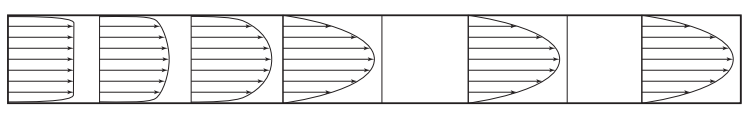
\includegraphics[width=\linewidth]{pic1.png}
	\caption{Схема формирования потока газа в трубе круглово сечения}
\end{wrapfigure}

\indent По мере продвижения  газа по	трубке	
картина распределения скоростей меняется, так как сила трения о стенку тормозит прилежащие к ней слои. Характерное для ламинарного	
течения параболическое распределение скоростей устанавливается на	
некотором расстоянии a от входа в трубку, которое зависит от радиуса трубки r и числа Рейнольдса по формуле: $$a\approx0,2r*Re$$\\

\subsection{Экспериментальная установка}

\begin{wrapfigure}{l}{0.5\linewidth}\label{pic:Pic2}
	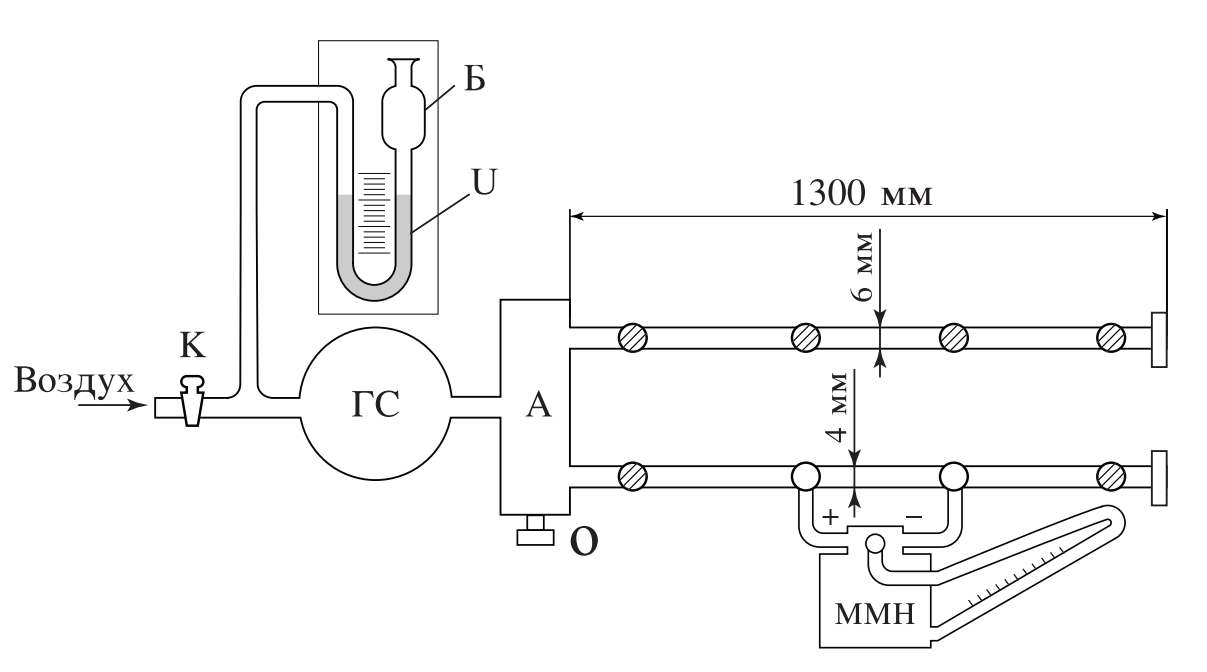
\includegraphics[width=\linewidth]{pic2.png}
	\caption{Схема установки для определения вязкости воздуха}

\end{wrapfigure}
Измерения производятся на экспериментальной установке, схема которой изображена на рис. 2. Поток воздуха под давлением, несколько превышающим атмосферное (на 5–7 см вод. ст.), через газовый счетчик ГС поступает в резервуар А, к которому припаяны тонкие металлические трубки.
\\[1ex]\
\indent Обе трубки на концах снабжены заглушками, не пропускающими воздух. Во время измерений заглушка открывается только на рабочей трубке; конец другой трубки должен быть плотно закрыт. Перед входом в газосчётчик поставлена U-образная трубка, наполовину заполненная водой. Она выполняет две задачи.
\\[1ex]\
\indent 
Первая - измерение давления газа на входе в газосчётчик. Вторая - предохранение газосчётчика от выхода из строя. Дело в том, что газосчётчик устойчиво работает, если давление газа на его входе не превышает 600 мм водяного столба. Высота U-образной трубки примерно 600 мм, поэтому, когда давление на входе в счётчик превышает 600 мм водяного столба,вода из U-образной трубки выплёскивается в защитный баллон Б и, создавая шум, привлекает к себе внимание экспериментатора. Такая ситуация часто создаётся в тех случаях, когда газ подают в систему при закрытых выходах измерительных трубок.

Для измерения давлений в трубках просверлен ряд миллиметровых отверстий. На время опыта к двум соседним отверстиям подсоединяется микроманометр, а остальные плотно закрываются завинчивающимися пробками. Подача воздуха в установку регулируется краном К.

\begin{wrapfigure}{r}{0.5\linewidth}
	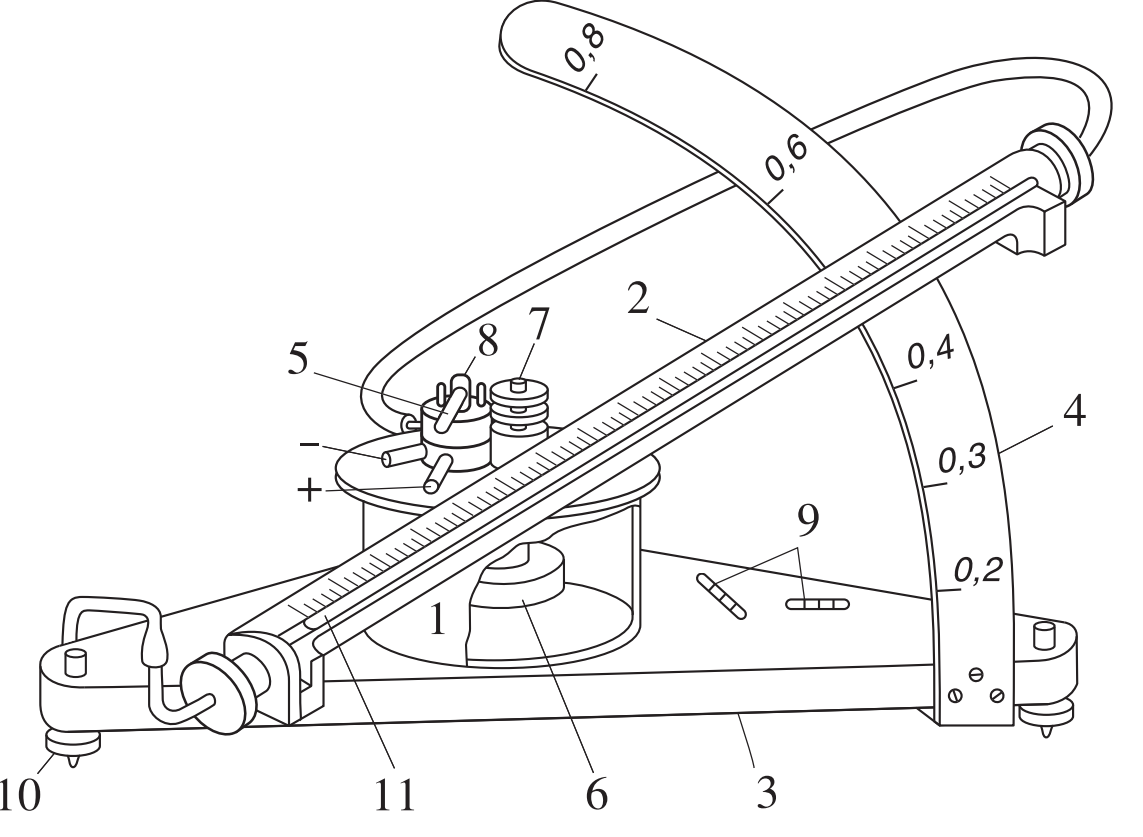
\includegraphics[width=\linewidth]{pic3.png}\label{pic:Pic3}
	\caption{Микрометрический манометр типа ММН}
\end{wrapfigure}
В работе применяется микроманометр типа ММН (рис. 3), позволяющий измерять разность давлений до 200 мм вод. ст. Для повышения чувствительности трубка манометра установлена в наклонном положении. Числа 0,2; 0,3; 0,4; 0,6 и 0,8(\textbf{В нашем случае - 0,2}) нанесенные на стойке 4, обозначают коэффициент, на который должны быть умножены показания манометра при данном наклоне, для получения давления в миллиметрах водяного столба. Рабочей жидкостью является этиловый спирт. Установка мениска жидкости на нуль шкалы производится путем изменения уровня спирта в сосуде 1 с помощью цилиндра 6. Глубина погружения цилиндра в спирт регулируется винтом 7.\\[1ex]\

\indent Микроманометр снабжен двумя уровнями 9, расположенными на плите 3 перпендикулярно один другому. Установка прибора по уровням производится двумя регулировочными ножками 10.

\begin{figure}
\begin{floatrow}
	 \ffigbox{\label{pic:Pic4}	\caption{Внешний вид
газового счетчика}}{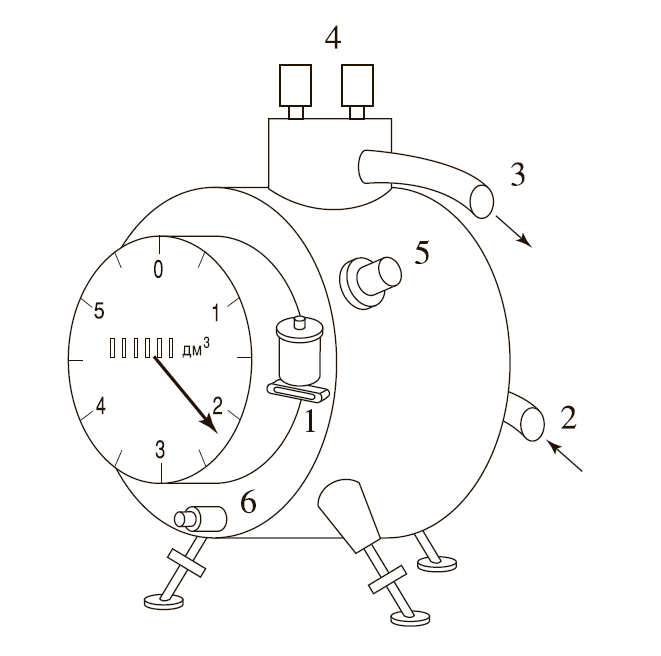
\includegraphics[width=\linewidth]{pic4.png}}
	
	\ffigbox{\label{pic:Pic5}\center \caption{Схема устройства газового
счетчика}}{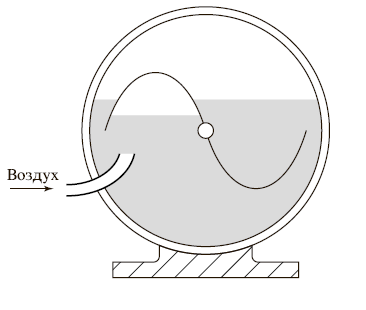
\includegraphics[width=\linewidth]{pic5.png}}

\end{floatrow}

\end{figure}

Газовый счетчик служит для измерения небольших количеств газа. Внешний вид его изображен на рис. 4. Корпус газового счетчика представляет собой цилиндрический баллон, на передней торцевой стенке которого находятся счетно-суммирующий механизм и шкала со стрелкой. Один оборот стрелки соответствует 5 л газа, прошедшего через счетчик.
\\[1ex]\
\indent
Газовый счетчик заливается водой до уровня, определяемого по во домерному устройству 1. Трубка 2 для входа газа расположена сзади счетчика, а трубка 3 для выхода газа наверху счетчика. Патрубки 4 предназначены для присоединения U-образного манометра, а патру бок 5 для установки термометра. Кран 6 служит для слива воды. Счетчик снабжен уровнем и регулировочными ножками для правильной установки.
\\[1ex]\
\indent
Принцип работы счетчика пояснен на рис. 5. На оси, проходящей по осевой линии цилиндра, жестко укреплены легкие чаши (для упрощения чертежа на рисунке изображены только две чаши). В чашу, находящуюся над трубкой 2, поступает воздух. Когда чаша наполняется воздухом, она всплывает, ее место занимает следующая, и т. д. Вращение оси передается счетно-суммирующему устройству.

\section{Ход работы}
\subsection{Поготовка}
\subsubsection{Оценим расстояние, на котором происходит формирование потока при ламинарном течении:}

\begin{table}[H]
    \begin{tabular}{|l|l|l|l|}
    \hline
    Трубка, № & $d_{\text{трубки}}$, mm & $a_{\text{посчитанное}}$, cm & $a_{\text{действительное}}$, cm \\ \hline
    1              &    3,85            &    38,5        &    81   \\[0.3ex]
    2              &    3               & 30             & 46      \\[0.3ex]
    3              & 2.6                & 26             & 40      \\ \hline
    \end{tabular}
    \caption {Таблица демонстрирующая, что наши измерения проводилось именно на участах ламинарного течения}
\end{table}


Давление, измеряемое \textbf{спиртовым} микроманометром, определяется по формуле:
$$P=K*h*9,80665 \text{ в нашем случае } K = 0.2$$

\subsection{Измерения}

\begin{table}[H]
\centering
\caption{Измерим вязкость воздуха. Для этого на Трубке №1 снимем зависимость  разности давлений от расхода газа}
\label{tab:tab1}
\begin{tabular}{|l|l|l|}
\hline
Q, литр/с & $\Delta$ p, mm & $\Delta p$, Pa \\ \hline
0,016 & 15 & 29,42 \\ [0.4ex]
0,032 & 29 & 56,88 \\[0.4ex]
0,053 & 46 & 90,22 \\[0.4ex]
0,07 & 64 & 125,53 \\[0.4ex]
0,09 & 83 & 162,79 \\[0.4ex]
0,09 & 95 & 186,33\\[0.4ex]
0,10 & 118 & 231,44 \\[0.4ex]
0,12 & 175 & 343,23 \\[0.4ex]
0,13 & 213 & 417,76 \\[0.4ex]
0,15 & 282 & 553,1 \\[0.4ex]
0,11 & 132 & 258,90 \\[0.4ex]
0,07 & 64 & 125,52 \\ \hline
\end{tabular}
\end{table}

\newpage
\subsection{Зависимость $\Delta$P = f(Q). Подсчет $Re$}
По полученным данным построим график $\Delta P$ = f(Q)


\begin{figure}[!h]
{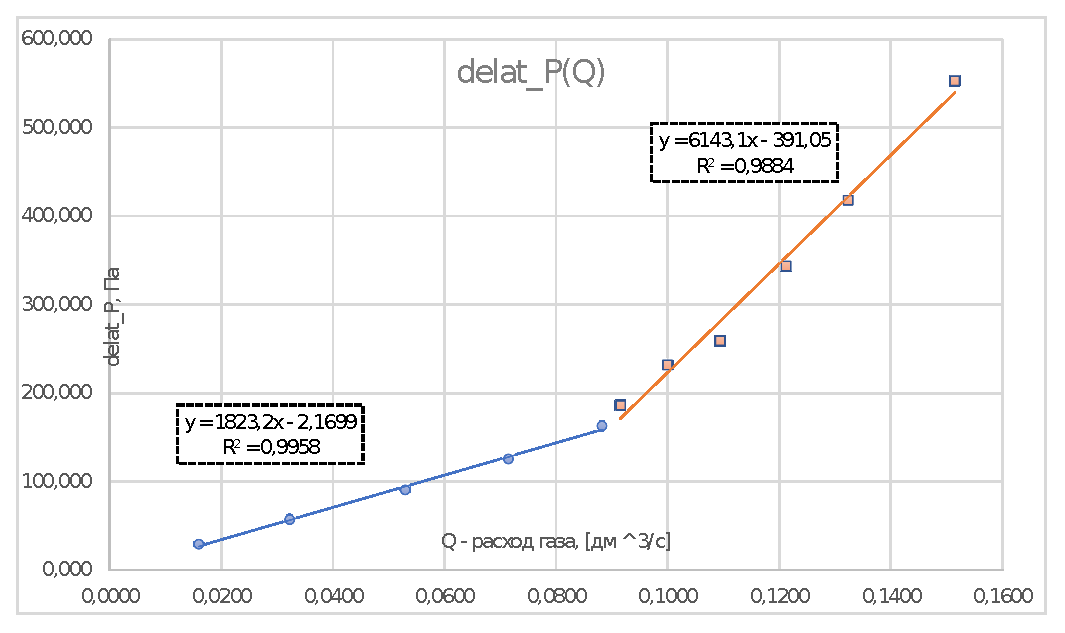
\includegraphics[width=1\linewidth]{graph1.eps}}
\caption{График зависимости $\Delta P$ от Q, для $d \approx 3,85 мм$(Трубка №1)}
\end{figure}


Выразим искомую вязкость через коэффициент наклона прямой $\alpha$
$$h=\eta*\frac{8l}{\pi r^4K*9,80665}Q=\alpha Q$$
$$\eta = \frac{\pi r^4 K*9,80665 \alpha}{8l}$$
$l=(50,0\pm0,1$) cм \\
$r=(1.925\pm0,03$) cм \\

\begin{tabular}{|c|}
\hline 
$\eta =(1,96)*10^{-5}$ кг*м/с \\ 
\hline 
\end{tabular} 
\ \\
\ \\
\ \\
Из графика видно, что ламинарный режим переходит в турбулентный на значениях $(9 \leftrightsquigarrow 10)*10^2 \ 10^{-2} \text{дм}^3/s$
$$Re=\frac{Qr\rho}{S\eta}$$
$Re=(980-1100)$
\ \\
\ \\
\begin{tabular}{|c|}
\hline 
\large{$Re=1040\pm60$}\\ 
\hline 
\end{tabular}
\ \\
\ \\
\subsection{Распределение давление внутри трубки}
При расходе, заведомо обеспечивающем ламинарность потока измерим распределение давления вдоль трубки:

\begin{table}[H]
\caption{Измерим разности давлений воздуха на различных участках Трубки №1}
\label{tab:tab2}

\begin{tabular}{|c|c|c|c|c|c|}
\hline 
l, см & 0 & 10,5 & 40,5 & 80,5 & 130,5 \\ 
\hline 
h, дел & 0 & 16 & 36 & 59 & 88 \\ 
\hline 
\end{tabular}
\end{table}

\begin{figure}[!h]
{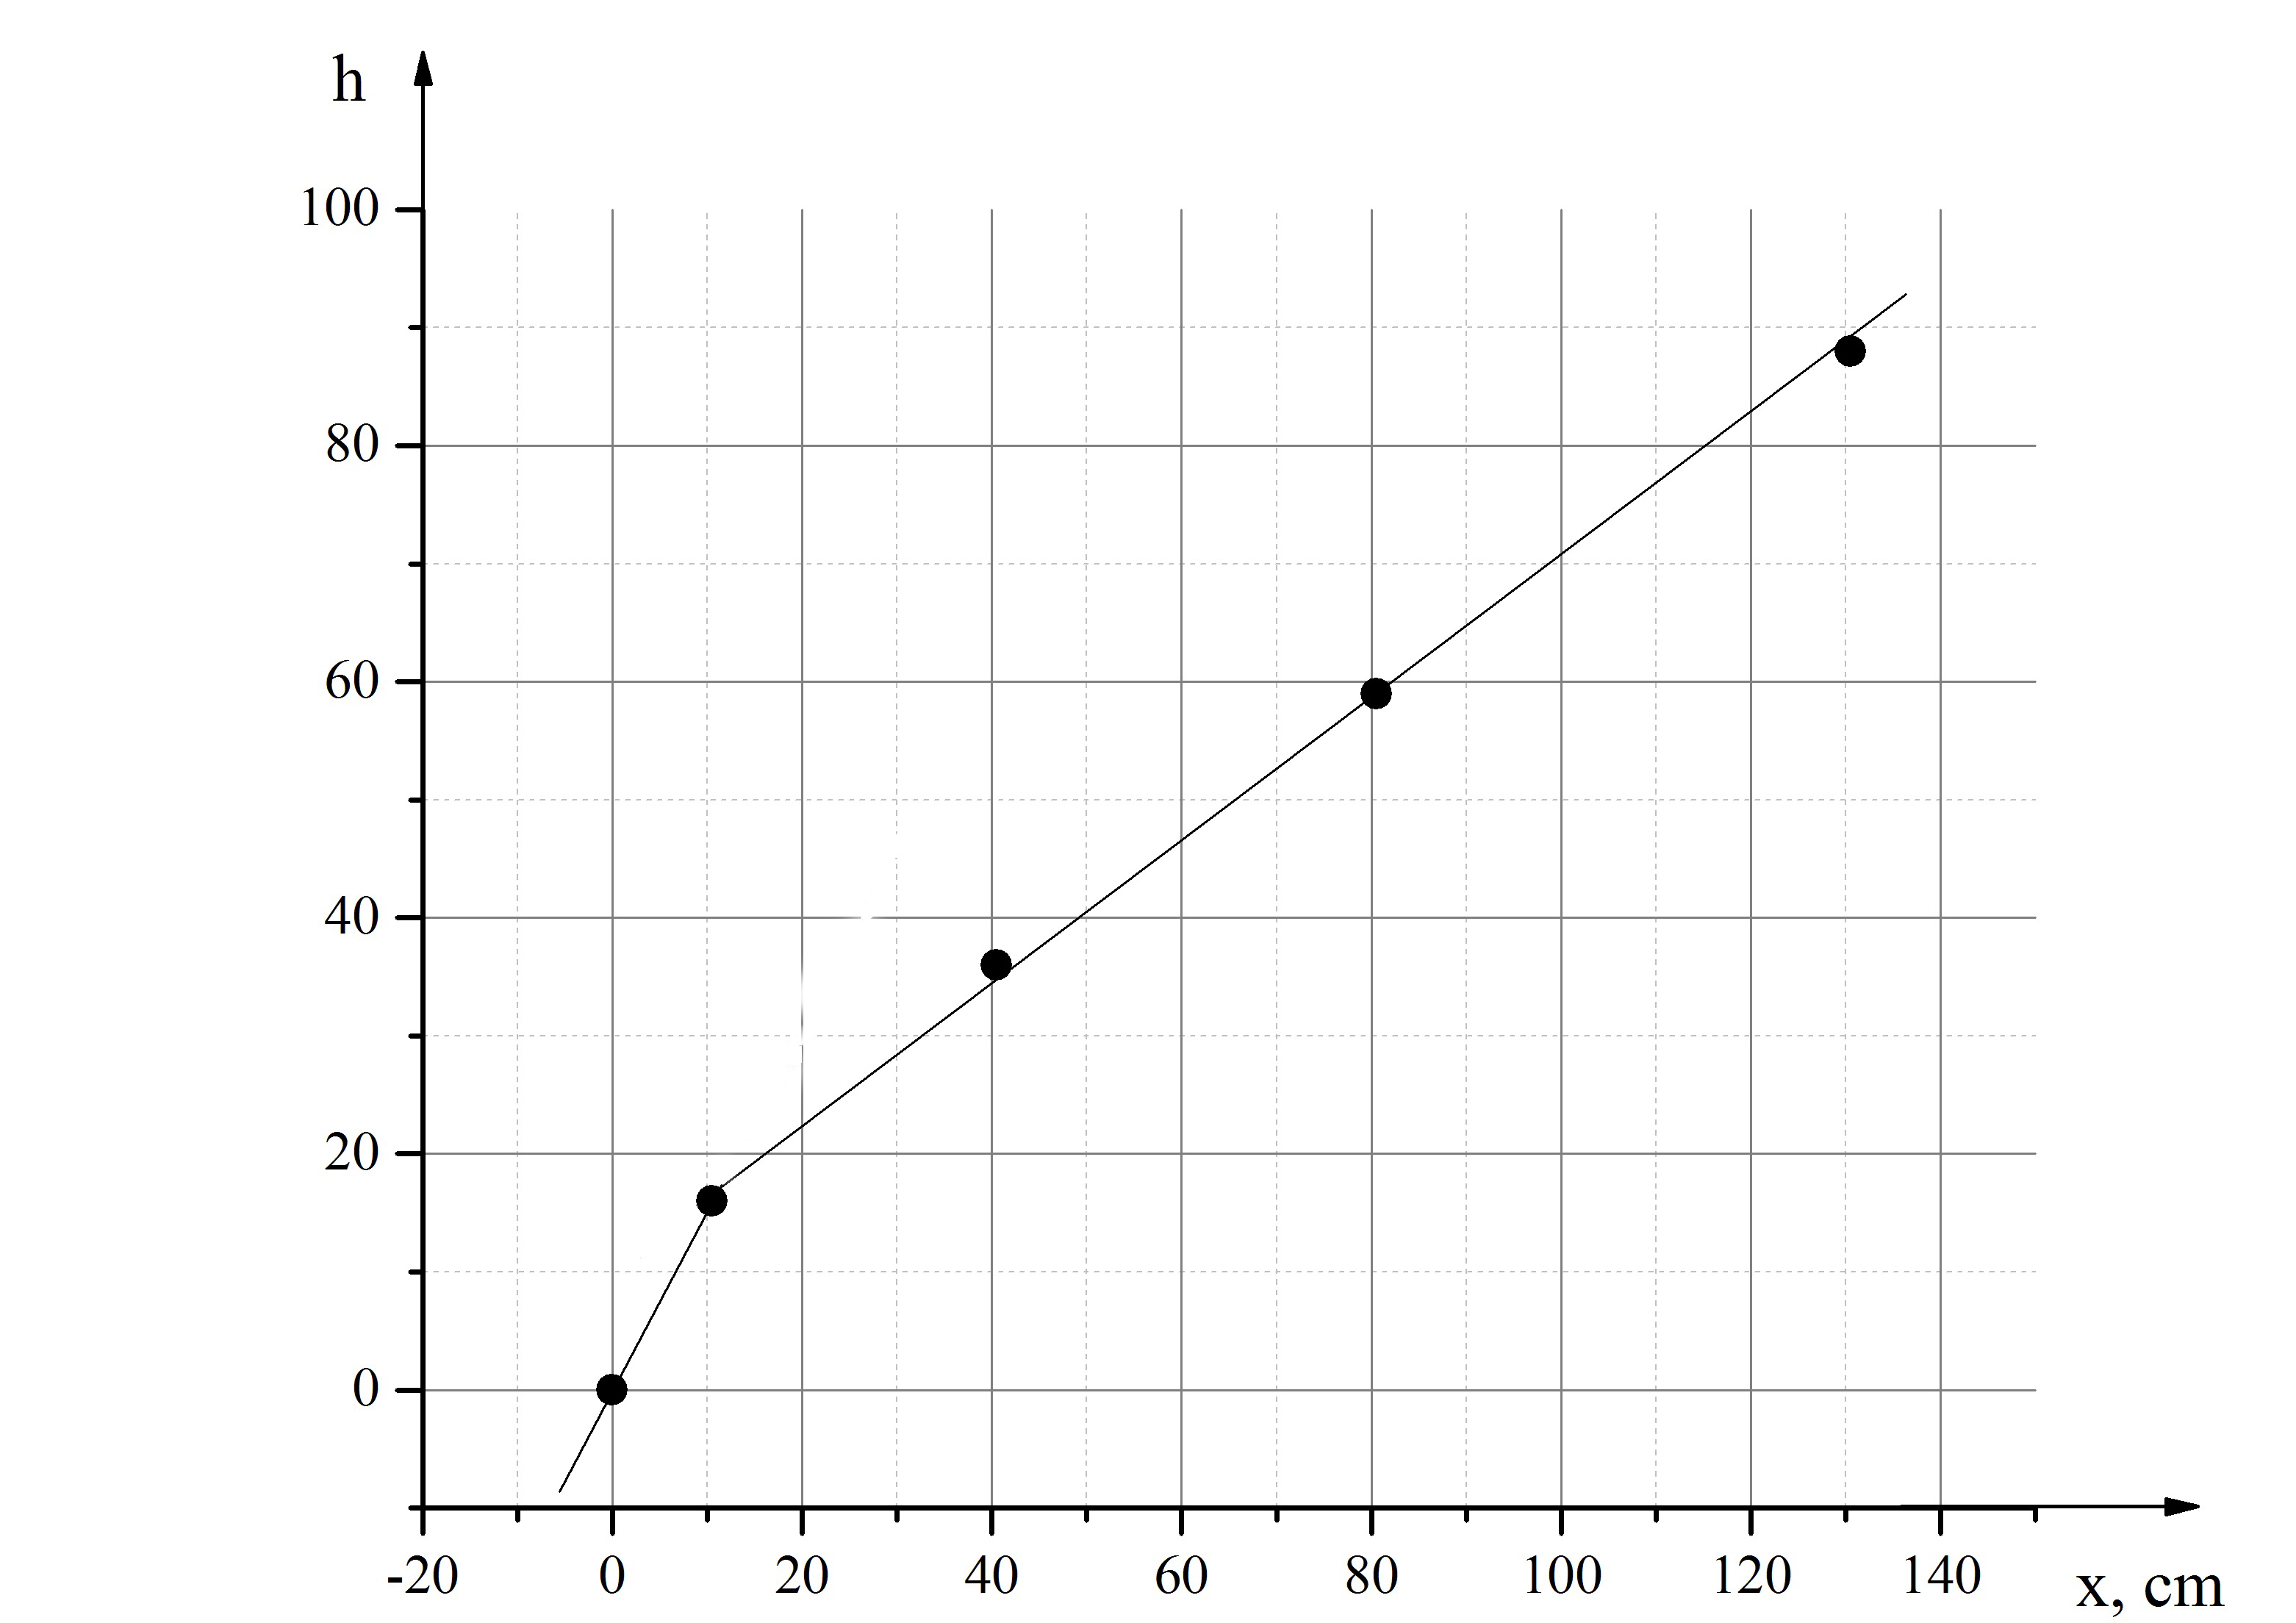
\includegraphics[width=1\linewidth]{Graph4.jpg}}
\caption{График зависимости давления(p) от расстояния(l)}
\end{figure}

\indent Из графика видно, что установление потока происходит еще на 1-ом участке длиной 10,5 см. Теоретические расчеты дали длину установления порядка 40 см. То есть оценка, полученная по формуле, гораздо более грубая, чем результат, который мы наблюдаем в эксперименте.

\newpage
\section{Обработка результатов}

\subsection{Измерения зависимости Q от P на разных трубках}

\subsubsection{Вывод необходимых формул}
\indent Проверим формулу Пуазейля. Для этого на концах двух труб снимем зависимость Q(P). Исходя из результатов предыдущего опыта можно утверждать, что поток на этих участках ламинарен, а значит имеет место формула: 
$$\frac{8l\eta Q}{\pi(P_1-P_2)}=r^n$$
Так как для каждой трубы поток \textit{ламинарен}:
\[\ln\Big(\dfrac {8l\eta}{\Pi}*k \Big) = n* \ln r \]


\indent Для всех трубок проведем измерения зависимости Q от P и обработаем их по формуле 
$$\frac{8l\eta Q}{\pi(P_1-P_2)}=r^n$$
$$\ln \Big(\frac{8l\eta Q}{\pi(P_1-P_2)} \Big) = n\ln r$$


\subsubsection{Измерения}
\begin{figure}[h]
\begin{floatrow}
	 \ffigbox{
	 \caption{Таблица измерений зависимости Q от P в Трубке №1 и Трубке №2 }
	 
\label{my-label}}{ \begin{tabular}{|l|l|l|l|}
\hline
C, $10^{11}$ & ln(C)  & r, mm & $\ln(r)$ \\ \hline
1,37                     & -25,01 & 1,93  & -6,253 \\
4,75                     & -23,77 & 2,63  & -5,943 \\ \hline
\end{tabular}}
	\ffigbox{\label{lab1}
	\caption{График зависимости Q = f(P), построенный в логарифмичеком масштабе}}
{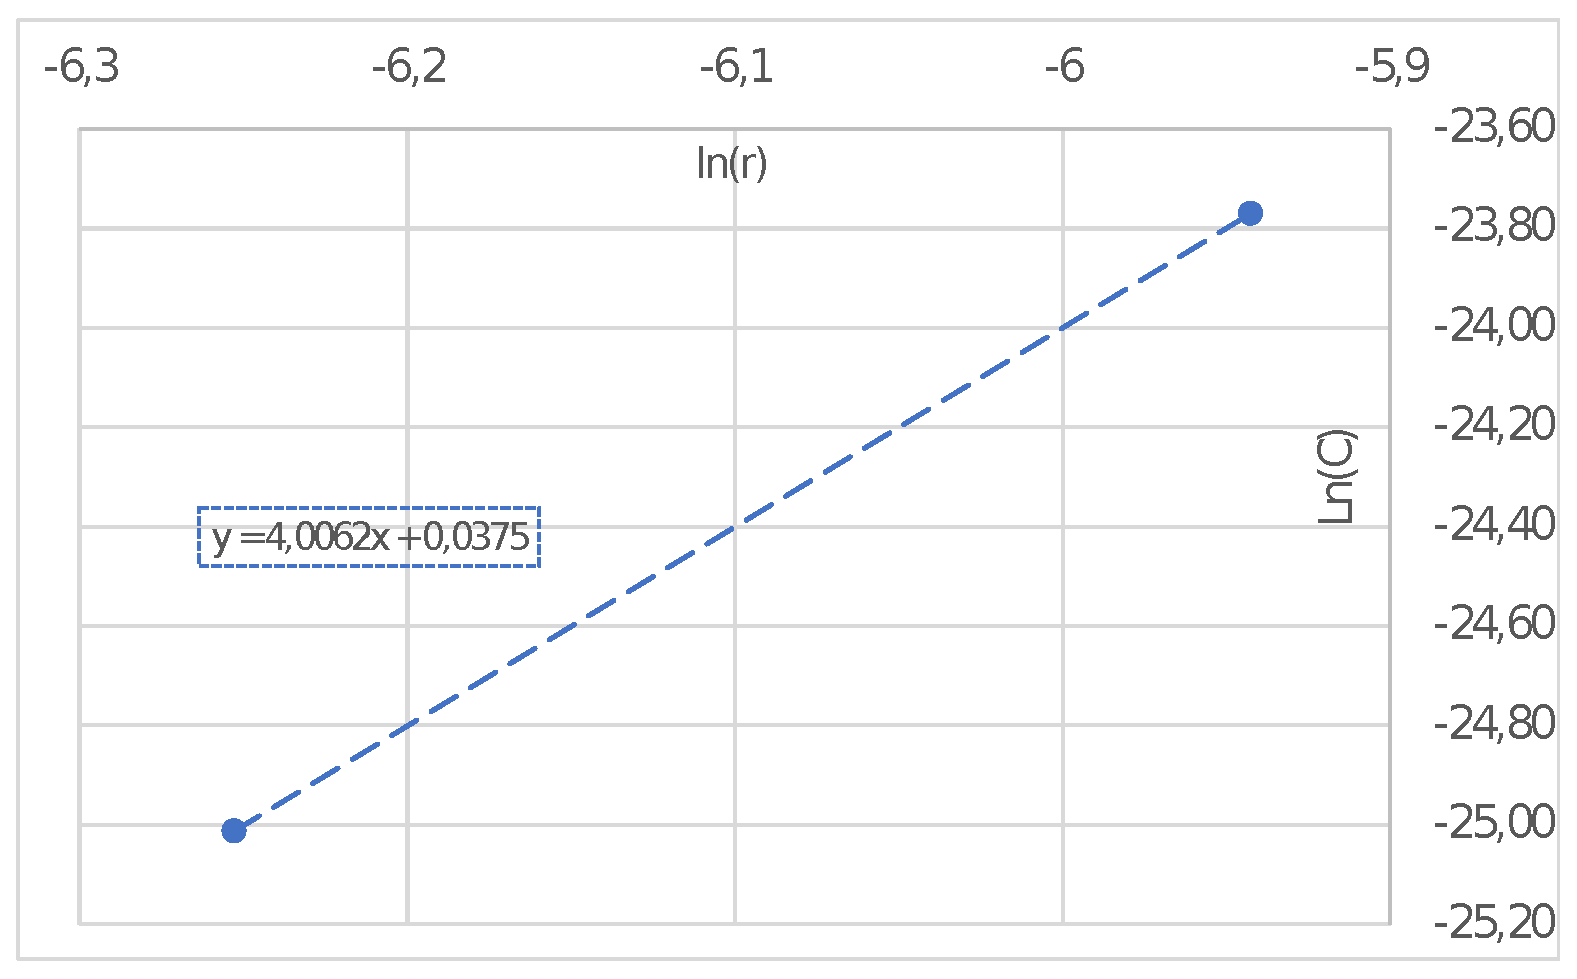
\includegraphics[width=1\linewidth]{graph2.eps}}

\end{floatrow}

\end{figure}

\indent Значение n - показателя $ r \approx 4$, что соответствует теории

\subsection{Погрешности}
	\subsubsection{При подсчете коэффициента линейной зависимости из графика $\Delta P (Q)$}
	\begin{equation}\label{eq:eq1} 
	\sigma_a \approx \dfrac{1}{\sqrt{n}} \sqrt{\dfrac{(<y^2>-<y>^2)}{(<x^2>-<x>^2 )} - a^2}
\end{equation}
	
\indent Тогда погрешность при измерении коэффициента вязкости $\eta$ :
\[\sigma_\eta = \eta*\sqrt{4\cdot\Big(\dfrac{\sigma_r}{r} \Big)^2 +\Big(\dfrac{\sigma_l}{l} \Big)^2 + \Big(\dfrac{\sigma_a}{a} \Big)^2 }\]

\indent В итоге:
	\[\sigma_a \approx 0,02 * 10^6\]
Значит $\eta=(\Pi*r^4)/8l*a :$
	\[\sigma_\eta \approx 0.1 * 10 ^{-5}\]

\subsubsection{При измерении Q = f(P) в логарифмическом масштабе}
	\indent Использую аналогичную формулу формулу(№\ref{eq:eq1}):
	\[\sigma\Big(\dfrac{Q}{\Delta P}\Big) \approx 1,051\]
\section{Вывод}	

\[\eta =(1,96)*10^{-5} \text{кг*м/с} \hspace{5ex} Re=1040\pm60 \hspace{5ex} n=4\pm 0,07\]

\begin{itemize}


\item На графике $\Delta P(Q)$ четко видно начало турбулентности и линейная зависимость на ламинарном участке.

\item Полученное экспериментально значение имеет небольшую относительную погрешность, лежит в пределах погрешности от табличного, что говорит об удачном проведении опыта.\\
Данная лабораторная работа поражает точностью результатов.(Схожестью теоретических и экспериментальных результатов)

\item Число Рейнольдса, полученное в результате опыта имеет соответствующее для переходного от ламинарного к турбулентному потоку значение.

\item Опытным путем установлен показатель степени $r \approx 4$.

\end{itemize}

\end{document}
